\noindent\begin{minipage}{7cm}
\begin{description}
\item[Objectif :] savoir trier une séquence.
\item[Syntaxe \python :] \mbox{}
\begin{Verbatim}
>>> t = [6,4,1,3,5,2]
>>> trier(t)
>>> t
[1, 2, 3, 4, 5, 6]
\end{Verbatim}
\end{description}
\end{minipage}
\mbox{}\hfill
\begin{minipage}{8cm}\footnotesize
$\displaystyle\left\downarrow
\begin{minipage}{3.5cm}
$\begin{array}{|c|ccccc|}
\hline
6 & 4 & 1 & 3 & 5 & 2 \\
\hline
\end{array}$
\vspace*{1mm}

$\begin{array}{|cc|cccc|}
\hline
\color{blue}\bf 4 & 6 & 1 & 3 & 5 & 2 \\
\hline
\end{array}$
\vspace*{1mm}

$\begin{array}{|ccc|ccc|}
\hline
\color{blue}\bf 1 & 4 & 6 & 3 & 5 & 2 \\
\hline
\end{array}$
\vspace*{1mm}

$\begin{array}{|cccc|cc|}
\hline
1 & \color{blue}\bf 3 & 4 & 6 & 5 & 2 \\
\hline
\end{array}$
\vspace*{1mm}

$\begin{array}{|ccccc|c|}
\hline
1 & 3 & 4 & \color{blue}\bf 5 & 6 & 2 \\
\hline
\end{array}$
\vspace*{1mm}

$\begin{array}{|cccccc|}
\hline
1 & \color{blue}\bf 2 & 3 & 4 & 5 & 6 \\
\hline
\end{array}$
\end{minipage}\right.$
\hfill
\begin{minipage}{3cm}
Tri de la liste\\ {\tt [6,4,1,3,5,2]}:\\
en gras, les valeurs insérées dans la partie
gauche à chaque éta\-pe.
\end{minipage}
\end{minipage}
%\begin{tabular}{c}
%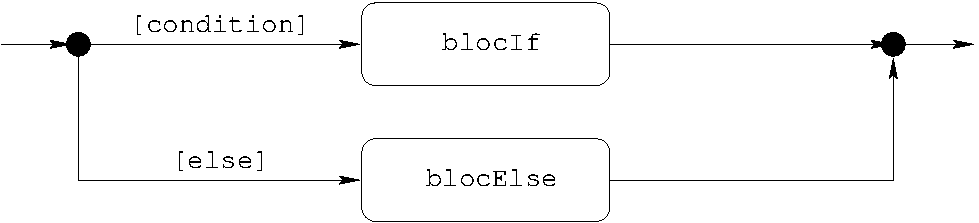
\includegraphics[width=6.5cm]{uml1.pdf}\\[3mm]
%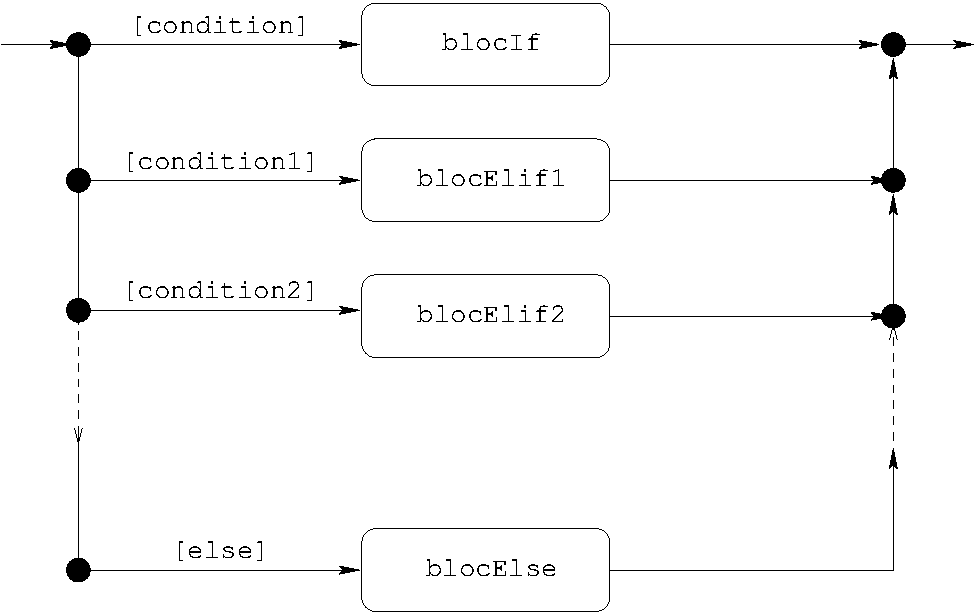
\includegraphics[width=6.5cm]{uml3.pdf}
%\end{tabular}

%-------------------------------------------------------------------------
\subsection{Exemple}
%-------------------------------------------------------------------------

\paragraph{Enoncé :} On cherche à trier un jeu de $n$ cartes selon les valeurs 
décroissantes des cartes et des couleurs ($\spadesuit > \heartsuit > \diamondsuit > \clubsuit$).\\
Exemple : 
A$\heartsuit$, $10\clubsuit$, $9\spadesuit$, $7\diamondsuit$, V$\spadesuit$, R$\clubsuit$, D$\heartsuit$, $7\heartsuit$
$\ \longrightarrow\ $ 
V$\spadesuit$, $9\spadesuit$, A$\heartsuit$, D$\heartsuit$, $7\heartsuit$, $7\diamondsuit$, R$\clubsuit$, $10\clubsuit$
\vspace*{3mm}

\noindent\begin{minipage}{9cm}
\paragraph{Méthode :} Prendre les cartes mélangées une à une sur la table, 
et former une « main » en insérant chaque carte saisie à sa place : on parle de tri par
insertion.

Dans le tri d'une séquence par insertion, on parcourt la séquence à trier du début à la fin. 
Au moment où on considère le $i^{\grave{e}me}$ élément, les éléments qui le précèdent sont déjà triés. Dans le cas du jeu de cartes, le $i^{\grave{e}me}$ élément est la carte saisie, les éléments précédents sont la main triée et les éléments suivants correspondent aux cartes encore mélangées sur la table.

\end{minipage}
\hfill
\begin{minipage}{6cm}
\centerline{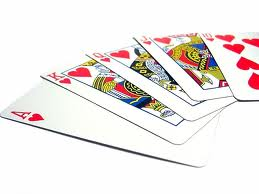
\includegraphics[width=6cm]{cartes-1.jpg}}
\end{minipage}




\paragraph{Questions :} \mbox{}

\begin{question}[« jeu de cartes » : tri par insertion]\mbox{}
On considère la séquence de 8 cartes suivante : A$\heartsuit$, $10\clubsuit$, $9\spadesuit$, $7\diamondsuit$, V$\spadesuit$, R$\clubsuit$, D$\heartsuit$, $7\heartsuit$. 
Décrire, étape par étape,
le passage de cette séquence à la séquence triée : V$\spadesuit$, $9\spadesuit$, A$\heartsuit$, D$\heartsuit$, $7\heartsuit$, $7\diamondsuit$, R$\clubsuit$, $10\clubsuit$,
par la méthode du tri par insertion.
\end{question}

\begin{question}[« jeu de cartes » : complexité]\mbox{}
\begin{enumerate}
\item Combien de comparaison effectuera-t-on en moyenne pour trier un jeu de $n$ cartes 
	par la méthode du tri par insertion ?
\item Si le jeu de $n$ cartes est déjà trié en ordre inverse, combien de comparaison 
	effectuera-t-on pour trier les cartes par la méthode du tri par insertion ?
\end{enumerate}
\end{question}

%-------------------------------------------------------------------------
\subsection{Généralisation}
%-------------------------------------------------------------------------
Dans la suite, nous supposerons qu'il existe une relation d'ordre total, 
entre les éléments de la liste à trier, notée $\leq$ et qui vérifie les propriétés 
habituelles de réflexivité, d'antisymétrie et de transitivité :
\begin{enumerate}
\item réflexivité : $x \leq x$
\item antisymétrie : $(x \leq y) \mbox{\tt\ and\ } (y \leq x) \Rightarrow x = y$
\item transitivit\'e : $(x \leq y) \mbox{\tt\ and\ } (y \leq z) \Rightarrow (x \leq z)$
\end{enumerate}


\begin{question}[relation d'ordre]
Définir une fonction \texttt{enOrdre} qui teste si une liste \texttt{t} est triée par ordre croissant de ses
éléments entre les rangs \texttt{debut} (inclus) et \texttt{fin} (inclus), 
en utilisant la relation d'ordre \texttt{<=} : \texttt{t[i-1] <= t[i] <= t[i+1]}.
\end{question}

Le tri par sélection d'une liste consiste à rechercher le minimum de la liste
à trier, de le mettre en début de liste en l'échangeant avec le premier élément
et de recommencer sur le reste de la liste.

\noindent\begin{minipage}{4cm}\footnotesize
$$\displaystyle\left\downarrow
\begin{minipage}{3.5cm}
$\begin{array}{|cccccc|}
\multicolumn{6}{c}{\mbox{\textbf{Tri par sélection}}}\\
\hline
6 & 4 & 1 & 3 & 5 & 2 \\
\hline
\end{array}$
\vspace*{1mm}

$\begin{array}{|cccccc|}
\hline
\color{blue}\bf 1 & 4 & \color{blue}\bf 6 & 3 & 5 & 2 \\
\hline
\end{array}$
\vspace*{1mm}

$\begin{array}{|cccccc|}
\hline
1 & \color{blue}\bf 2 & 6 & 3 & 5 & \color{blue}\bf 4 \\
\hline
\end{array}$
\vspace*{1mm}

$\begin{array}{|cccccc|}
\hline
1 & 2 & \color{blue}\bf 3 & \color{blue}\bf 6 & 5 & 4 \\
\hline
\end{array}$
\vspace*{1mm}

$\begin{array}{|cccccc|}
\hline
1 & 2 & 3 & \color{blue}\bf 4 & 5 & \color{blue}\bf 6 \\
\hline
\end{array}$
\vspace*{1mm}

$\begin{array}{|cccccc|}
\hline
1 & 2 & 3 & 4 & \color{blue}\bf 5 & 6 \\
\hline
\end{array}$
\vspace*{1mm}

$\begin{array}{|cccccc|}
\hline
1 & 2 & 3 & 4 & 5 & \color{blue}\bf 6 \\
\hline
\multicolumn{6}{p{2.75cm}}{}\\
\multicolumn{6}{p{2.75cm}}{en gras, les valeurs échan\-gées à chaque éta\-pe}
\end{array}$
\end{minipage}\right.$$
\end{minipage}
\hfill
\begin{minipage}{11cm}\footnotesize
\begin{lstlisting}
def triSelection(t,debut,fin):
    assert type(t) is list
    assert 0 <= debut <= fin < len(t)
    if debut < fin:
        mini = minimum(t,debut,fin)
        t[debut],t[mini] = t[mini],t[debut]
        triSelection(t,debut+1,fin)
    return
\end{lstlisting}
\end{minipage}

\begin{question}[tri par sélection]\mbox{}
\begin{enumerate}
\item Définir la fonction \texttt{minimum} qui retourne le rang du plus petit élément 
	de la séquence \texttt{t} entre les rangs \texttt{debut} (inclus) et \texttt{fin} (inclus).
\item Proposer une version itérative de la fonction \texttt{triSelection} 
	qui trie la liste {\tt t} par ordre croissant entre les rangs \texttt{debut} (inclus) 
	et \texttt{fin} (inclus).
\end{enumerate}

\end{question}

Le principe du tri rapide  est le suivant : on partage la 
liste à trier en deux sous-listes telles que tous les éléments de la première 
soient inférieurs à tous les éléments de la seconde.
Pour partager la liste en deux sous-listes, on choisit un des éléments de la liste
(par exemple le premier) comme pivot. On construit alors une sous-liste
avec tous les éléments inférieurs ou égaux à ce pivot et une sous-liste avec 
tous les éléments supérieurs au pivot.
On trie les deux sous-listes selon le même processus jusqu'à avoir des sous-listes 
réduites à un seul élément.


\noindent\begin{minipage}{4cm}\footnotesize
$$\displaystyle\left\downarrow
\begin{minipage}{3.5cm}
$\begin{array}{|c|ccccc|}
\multicolumn{6}{c}{\mbox{\textbf{Tri rapide}}}\\
\hline
6 & 4 & 1 & 3 & 5 & 2 \\
\hline
\end{array}$
\vspace*{1mm}

$\begin{array}{|ccccc|c}
\cline{1-5}
2 & 4 & 1 & 3 & 5 & \color{blue}\bf 6\\
\cline{1-5}
\end{array}$
\vspace*{1mm}

$\begin{array}{|c|c|ccc|c}
\cline{1-1}\cline{3-5}
1 & \color{blue}\bf 2 & 4 & 3 & 5 & 6\\
\cline{1-1}\cline{3-5}
\end{array}$
\vspace*{1mm}

$\begin{array}{cc|c|c|c|c}
\cline{3-3}\cline{5-5}
1 & 2 & 3 & \color{blue}\bf 4 & 5 & 6 \\
\cline{3-3}\cline{5-5}
\end{array}$
\vspace*{1mm}

$\begin{array}{cccccc}
1 & 2 & 3 & 4 & 5 & 6 \\
\multicolumn{6}{p{2.75cm}}{}\\
\multicolumn{6}{p{2.75cm}}{en gras, les valeurs des pivots à chaque étape}
\end{array}$
\end{minipage}\right.$$
\end{minipage}
\hfill
\begin{minipage}{11cm}\footnotesize
\begin{lstlisting}
def triRapide(t,debut,fin):
    assert type(t) is list
    assert 0 <= debut 
    assert fin <= len(t)
    if debut < fin:
        pivot = t[debut]
        place = partition(t,debut,fin,pivot)
        triRapide(t,debut,place-1)
        triRapide(t,place+1,fin)
    return
\end{lstlisting}
\end{minipage}
\vspace*{2mm}

Pour partitionner la liste, on utilise 2 compteurs {\tt inf} et {\tt sup} qui partent des
2 extrémités de la liste en évoluant l'un vers l'autre.
Le compteur de gauche {\tt inf} part du début de la liste et lorsqu'il atteint un élément 
supérieur au pivot, on arrête sa progression. De même, le compteur de droite {\tt sup}
part de la fin de la liste et s'arrête lorsqu'il atteint un élément inférieur au pivot.
On échange alors ces deux éléments ({\tt t[sup],t[inf] = t[inf],t[sup]}) puis on continue
à faire progresser les compteurs et à faire des échanges jusqu'à ce que les compteurs se
croisent.

\begin{question}[tri rapide]\mbox{}
\begin{enumerate}
\item Définir la fonction \texttt{partition} qui partitionne la liste \texttt{t} entre les 
	rangs \texttt{debut} (inclus) et \texttt{fin} (inclus) par rapport au \texttt{pivot}.
\item Vérifier le bon fonctionnement de la version récursive de la fonction
	\texttt{triRapide} qui trie la liste \texttt{t} par ordre croissant entre les rangs
	\texttt{debut} (inclus) et \texttt{fin} (inclus).
\end{enumerate}
\end{question}

%-------------------------------------------------------------------------
\subsection{Applications}
%-------------------------------------------------------------------------
\begin{question}[tri bulles]\mbox{}
Dans le tri bulles, on parcourt la liste en commençant par la fin, 
en effectuant un échange à chaque fois que l'on trouve deux éléments 
successifs qui ne sont pas dans le bon ordre.
\begin{enumerate}
\item Définir une procédure \texttt{triBulles} qui trie une liste \texttt{t} par ordre 
	croissant entre les rangs \texttt{debut} (inclus) et \texttt{fin} (inclus) 
	selon la méthode du tri bulles.
\item Évaluer la complexité en nombre de comparaisons du tri bulles.
\end{enumerate}
\end{question}

\begin{question}[tri fusion]\mbox{}
Dans le tri fusion, on partage la liste à trier en deux sous-listes que l'on trie,
puis on interclasse (on fusionne) ces deux sous-listes.

Définir une procédure \texttt{triFusion} qui trie une liste \texttt{t} par ordre 
	croissant entre les rangs \texttt{debut} (inclus) et \texttt{fin} (inclus) 
	selon la méthode du tri fusion.
\end{question}


%-------------------------------------------------------------------------
%\newpage
\subsection{Entraînement}
%-------------------------------------------------------------------------

%-------------------------------------------------------------------------
\subsubsection{Enoncé}
%-------------------------------------------------------------------------

\paragraph{Objectif :} trier un annuaire selon différents critères, l'annuaire étant
représenté par une liste de quadruplets \texttt{(nom, age, ville, téléphone)}.\\
Exemple d'annuaire :
\begin{minipage}[t]{7cm}
\begin{Verbatim}
item1 = ('dupont', 23, 'brest', '06789656')
item2 = ('abgral', 61, 'lille', '06231298')
item3 = ('dupont', 23, 'brest', '02989656')
item4 = ('abgral', 67, 'brest', '06556438')
item5 = ('martin', 38, 'paris', '01674523')
item6 = ('abgral', 67, 'lille', '06231298')

annuaire = [item1, item2, item3, item4, item5, item6]
\end{Verbatim}
\end{minipage}

\paragraph{Méthode :} utiliser un algorithme de tri (sélection, bulles, insertion, fusion ou rapide).

\paragraph{Vérification :} vérifier à l'aide de différents annuaires et différents critères.

%-------------------------------------------------------------------------
\subsubsection{Exemple}
%-------------------------------------------------------------------------
Soit à trier un jeu de cartes stocké sous la forme d'une liste de couples 
{\tt (couleur,valeur)} où la valeur est un entier compris entre 2 et 14 
(valet = 11, dame = 12, roi = 13 et as = 14) et la couleur un autre entier tel que 
$\spadesuit = 4, \heartsuit = 3,  \diamondsuit = 2 \mbox{ et } \clubsuit = 1$.\\
Ainsi le jeu 
A$\heartsuit$, $10\clubsuit$, $9\spadesuit$, $7\diamondsuit$, V$\spadesuit$, R$\clubsuit$, D$\heartsuit$, $7\heartsuit$ est représenté par la liste 
{\tt [(3,14), (1,10), (4,9), (2,7), (4,11), (1,13), (3,12), (3,7)]}.



\noindent\begin{minipage}[t]{4.5cm}
\paragraph{Méthode :} On utilise un tri par insertion où la fonction \texttt{cmp}
de comparaison est passée en argument. Par défaut, le tri est effectué par ordre croissant 
des éléments :
\texttt{cmp = (lambda x,y : x < y)} .
\end{minipage}
\hfill
\begin{minipage}[t]{11cm}\footnotesize
\begin{lstlisting}
def triInsertion(t,cmp=(lambda x,y : x < y)) :
    assert type(t) is list
    for i in range(1,len(t)):
        x = t[i]
        k = i
        for j in range(i-1,-1,-1):
            if not cmp(t[j],x) :
                k = k-1
                t[j+1] = t[j]
        t[k] = x
    return
\end{lstlisting}
\end{minipage}

\paragraph{Résultat :} Il suffit ici d'appeler la fonction de tri avec la liste \texttt{t} de cartes voulue
en effectuant le tri par ordre décroissant des éléments : \texttt{cmp = (lambda x,y : x > y)}.
\vspace*{3mm}

\noindent \texttt{t = [A$\heartsuit$, 10$\clubsuit$, 9$\spadesuit$, 7$\diamondsuit$, V$\spadesuit$, R$\clubsuit$, D$\heartsuit$, 7$\heartsuit$]}
\begin{Verbatim}
>>> t = [(3,14), (1,10), (4,9), (2,7), (4,11), (1,13), (3,12), (3,7)]
>>> triInsertion(t,(lambda x,y : x > y))
>>> t
[(4, 11), (4, 9), (3, 14), (3, 12), (3, 7), (2, 7), (1, 13), (1, 10)]
\end{Verbatim}
\texttt{t = [V$\spadesuit$, 9$\spadesuit$, A$\heartsuit$, D$\heartsuit$, 7$\heartsuit$, 7$\diamondsuit$, R$\clubsuit$, 10$\clubsuit$]}

\paragraph{Vérifications :} la fonction sera testée avec différents jeux de cartes.
\begin{enumerate}
\item \texttt{t = []}
\begin{Verbatim}
>>> t = []
>>> triInsertion(t,(lambda x,y : x > y))
>>> t
[]
\end{Verbatim}
\item \texttt{t = [A$\heartsuit$, A$\clubsuit$, A$\spadesuit$, A$\diamondsuit$]}
\begin{Verbatim}
>>> t = [(3,14), (1,14), (4,14), (2,14)]
>>> triInsertion(t,(lambda x,y : x > y))
>>> t
[(4, 14), (3, 14), (2, 14), (1, 14)]
\end{Verbatim}

\item \texttt{t = [3$\clubsuit$, 5$\clubsuit$, 8$\clubsuit$, 9$\clubsuit$, R$\clubsuit$]}
\begin{Verbatim}
>>> t = [(1,3), (1,5), (1,8), (1,9), (1,13)]
>>> triInsertion(t,(lambda x,y : x > y))
>>> t
[(1, 13), (1, 9), (1, 8), (1, 5), (1, 3)]
\end{Verbatim}

\item \texttt{t = [R$\clubsuit$, 9$\clubsuit$, 8$\clubsuit$, 5$\clubsuit$, 3$\clubsuit$]}
\begin{Verbatim}
>>> t = [(1,13), (1,9), (1,8), (1,5), (1,3)]
>>> triInsertion(t,(lambda x,y : x > y))
>>> t
[(1, 13), (1, 9), (1, 8), (1, 5), (1, 3)]
\end{Verbatim}
\end{enumerate}

%-------------------------------------------------------------------------
\subsubsection{Questions}
%-------------------------------------------------------------------------
Un annuaire est représenté ici par une liste de quadruplets 
\texttt{(nom, age, ville, téléphone)}.\\
Exemple d'annuaire :
\begin{minipage}[t]{7cm}
\begin{Verbatim}
item1 = ('dupont', 23, 'brest', '06789656')
item2 = ('abgral', 61, 'lille', '06231298')
item3 = ('dupont', 23, 'brest', '02989656')
item4 = ('abgral', 67, 'brest', '06556438')
item5 = ('martin', 38, 'paris', '01674523')
item6 = ('abgral', 67, 'lille', '06231298')

annuaire = [item1, item2, item3, item4, item5, item6]
\end{Verbatim}
\end{minipage}
\vspace*{3mm}

Trier l'annuaire, par ordre croissant ou décroissant, selon des critères donnés 
par une liste des clés successives. 
L'ordre des critères est précisé par une liste des rangs successifs des champs du quadruplet
\texttt{(nom, age, ville, téléphone)}. Par exemple, la liste \texttt{[3,0,2,1]} indique
qu'il faut d'abord (clé primaire) trier selon les numéros de téléphone (champ \no 3 dans le quadruplet), puis (clé secondaire) selon les noms (champ \no 0 dans le quadruplet), 
puis selon la ville (champ \no 2 dans le quadruplet) et enfin selon les âges 
(champ \no 1 dans le quadruplet).

\noindent
\begin{minipage}[t]{7cm}
\begin{enumerate}
\item \texttt{cles = [2,0,1,3]}, croissant
\item \texttt{cles = [2,0,3,1]}, croissant
\item \texttt{cles = [2,1,0,3]}, croissant
\item \texttt{cles = [2,1,3,0]}, croissant
\item \texttt{cles = [2,3,0,1]}, croissant
\item \texttt{cles = [2,3,1,0]}, croissant
\item \texttt{cles = [3,0,1,2]}, croissant
\item \texttt{cles = [3,0,2,1]}, croissant
\item \texttt{cles = [3,1,0,2]}, croissant
\item \texttt{cles = [3,1,2,0]}, croissant
\item \texttt{cles = [3,2,0,1]}, croissant
\item \texttt{cles = [3,2,1,0]}, croissant
\end{enumerate}
\end{minipage}
\hfill
\begin{minipage}[t]{7cm}
\begin{enumerate}\setcounter{enumi}{12}
\item \texttt{cles = [0,1,2,3]}, décroissant
\item \texttt{cles = [0,1,3,2]}, décroissant
\item \texttt{cles = [0,2,1,3]}, décroissant
\item \texttt{cles = [0,2,3,1]}, décroissant
\item \texttt{cles = [0,3,1,2]}, décroissant
\item \texttt{cles = [0,3,2,1]}, décroissant
\item \texttt{cles = [1,0,2,3]}, décroissant
\item \texttt{cles = [1,0,3,2]}, décroissant
\item \texttt{cles = [1,2,0,3]}, décroissant
\item \texttt{cles = [1,2,3,0]}, décroissant
\item \texttt{cles = [1,3,0,2]}, décroissant
\item \texttt{cles = [1,3,2,0]}, décroissant
\end{enumerate}
\end{minipage}

%-------------------------------------------------------------------------
\subsection{Révisions}
%-------------------------------------------------------------------------

$$\begin{tabular}{|ll@{ : }l|}
\hline
\textbf{Cours} & \cite{cours} & chapitre 4, section 4.4 \\
\textbf{TD}    & \cite{td}    & exercices 4.15 à 4.19, 4.28 \\
\hline
\end{tabular}$$
